\documentclass{beamer}

\usepackage[utf8]{inputenc}
\usepackage[backend=biber,sorting=none,hyperref]{biblatex}
\usepackage{mathtools}
\usepackage{dsfont}
\usepackage{tikz}
\usetikzlibrary{topaths,calc,tikzmark}
\usepackage{algorithm2e}
\usepackage{pgfgantt}
\usepackage{marginnote}
\usepackage{marvosym}
\usepackage[marginpar]{todo}
\usepackage{pgfgantt}
\usepackage{textcomp}
\usepackage{subcaption}
\usepackage[T1]{fontenc}
\usepackage{inconsolata}
\usepackage{minted}
\usepackage{cprotect}
\usepackage[symbol]{footmisc}

\renewcommand{\thefootnote}{\fnsymbol{footnote}}

\title{Wordlength inference in the Spade HDL}
\subtitle{\say{Seven implementations of wordlength inference and one implementation that actually works}\\ or \say{A fishy situation}}
\author{Edvard Thörnros}
\institute{Department of Electrical Engineering at Linköping University}
\date{}

\addbibresource{thesis.bib}

\newcommand{\say}[1]{``#1''}


\usetheme{metropolis}

\begin{document}

\begin{frame}
\titlepage
\end{frame}

\begin{frame}
\frametitle{Outline}
\tableofcontents
\end{frame}

\section{The Problem}

\begin{frame}
\frametitle{The Spade programming language}
\begin{center}

\includegraphics[height=5em]{figures/spadefish.png}
\end{center}
\begin{block}{Spade}
A hardware description language inspired by modern software languages.
\end{block}
Developed here at LiU. Has cute mascot.
\end{frame}


\begin{frame}[containsverbatim]
\frametitle{A Spade-program}
\begin{center}
\begin{minted}{rust}
fn f(a: int<3>) -> int<4> {
  a + 2
}
\end{minted}
\end{center}
\vspace{1em}
A function where we add 2 to the argument. The argument has 3 bits of precision and the return value has 4 bits.
\end{frame}

\begin{frame}[containsverbatim]
\frametitle{Another Spade-program}
\begin{center}
\begin{minted}{rust}
fn f(a: int<3>) -> int<4> {
  a + 1 + 1
}
\end{minted}
\end{center}
\vspace{1em}
A function where we add 1 two times to the argument. The argument has 3 bits of precision and the return value has 4 bits.
\end{frame}

\begin{frame}[containsverbatim]
\frametitle{PANIK!}
\begin{minted}[fontsize=\footnotesize]{text}
error: Type error
  |- src/simple_fault.spade:1:27
  |
1 |   fn f(a: int<3>) -> int<4> {
  |                      ------ int<4> type specified here
  | |---------------------------^
2 | |   a + 1 + 1
3 | | }
  | |-^ Found type int<5>
  |
  = Expected: 4
  =       in: int<4>
  =      Got: 5
  =       in: int<5>

Error: aborting due to previous error
\end{minted}
\end{frame}

\begin{frame}
\frametitle{Solution?}
\begin{block}{Solution?}
Just forbid unnecessary additions. Thanks for coming!
\end{block}
\pause
\begin{alertblock}{Unless?}
\textit{Actually} a symptom of a problem that is much deeper but is tricky.
\end{alertblock}
\end{frame}

\section{Background}

\begin{frame}[containsverbatim]
A breif look at compilers, typesystems and some basics in self validating numeric methods.
\end{frame}

\begin{frame}[containsverbatim]
\frametitle{Compiler Overview}
\begin{figure}[h!]
\begin{center}
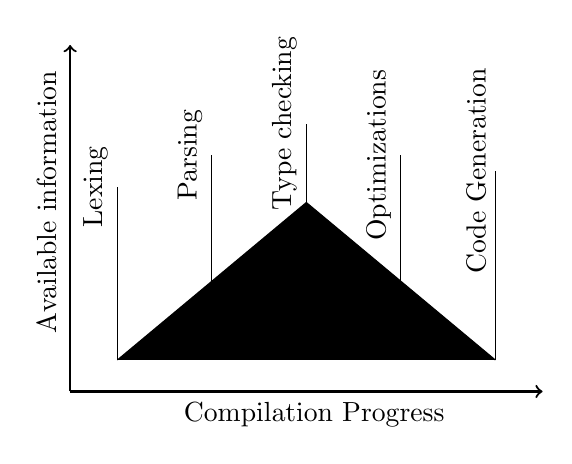
\begin{tikzpicture}[xscale=3, yscale=2]
\draw[->, thick] (-0.2,-0.2) -- (-0.2,2.0) node[xshift=-0.3cm, yshift=-0.2cm, left, rotate=90] {Available information};
\draw[->, thick] (-0.2,-0.2) -- (1.8,-0.2) node[xshift=-2.9cm, below] {Compilation Progress};
\draw (0.0,0) -- (0.0,1.1) node[above, rotate=90] {Lexing};
\draw (0.4,0) -- (0.4,1.3) node[above, rotate=90] {Parsing};
\draw (0.8,0) -- (0.8,1.5) node[above, rotate=90] {Type checking};
\draw (1.2,0) -- (1.2,1.3) node[above, rotate=90] {Optimizations};
\draw (1.6,0) -- (1.6,1.2) node[above, rotate=90] {Code Generation};
% horizontal line
\filldraw[color=black, fill=black] (0,0) -- (0.8,1.0) -- (1.6,0);
\end{tikzpicture}
\end{center}
\end{figure}
\end{frame}

\begin{frame}
\begin{figure}[h!]
  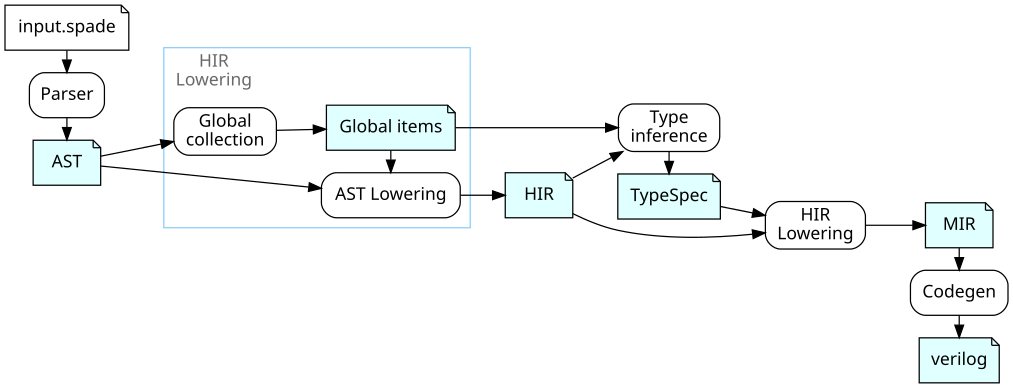
\includegraphics[width=\textwidth]{figures/architecture.png}
  \label{figArch}
\end{figure}
\end{frame}

\begin{frame}[containsverbatim]
\frametitle{Basics About Parsing}
\begin{minted}[]{bnf}
<expr> ::= <num> | <expr> + <expr>

<num>  ::= 1 | 2 | 3
\end{minted}
\end{frame}

\begin{frame}[containsverbatim]
\frametitle{Basics About Parsing}
\begin{verbatim}
  <expr> -> <expr> + <expr>
         -> <expr> + <expr> + <expr>
         -> <expr> + <expr> + <num>
         -> <expr> + <expr> + 1
         -> <expr> + <num> + 1
         -> <expr> + 2 + 1
         -> <num> + 2 + 1
         -> 3 + 2 + 1
\end{verbatim}
\end{frame}


\begin{frame}[containsverbatim]
\frametitle{Parse Trees}
\large
\centering
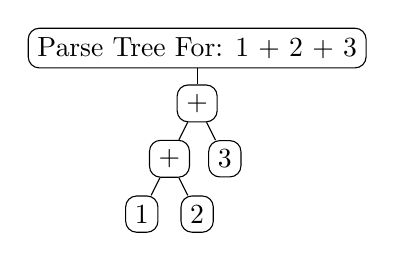
\begin{tikzpicture}[
  sibling distance=2em,
  level distance=2em,
  every node/.style = {shape=rectangle, rounded corners, draw, align=center}
]
  \node {Parse Tree For: 1 + 2 + 3}
          child {node {+}
            child {node {+}
              child {node {1}}
              child {node {2}}
            }
            child {node {3}}
          };
\end{tikzpicture}
\end{frame}

\subsection{Some Spade-Syntax}

\begin{frame}[containsverbatim]
\frametitle{Spade Example Program A}
\large
\centering
\begin{minted}[]{rust}
fn calculate(x: int<5>) -> int<7> {
  let partial_result: int<3> = some_function(3);
  x + 1 * 2 - partial_result
}
\end{minted}
\end{frame}

\begin{frame}[containsverbatim]
\frametitle{Spade Example Program B}
\large
\centering
\begin{minted}[]{rust}
fn generics<#A, #B, T>(x: int<A>, t: T) -> int<B> {
  if t == t {
    x + x
  } else {
    0
  }
}
\end{minted}
\end{frame}

\begin{frame}[containsverbatim]
\frametitle{Nice Spade Properties}
\begin{itemize}
  \item Little mutable state (*)
  \item No loops
  \item Damas-Hindley-Milner
\end{itemize}
\end{frame}

\subsection{The Spade Typesystem}

\begin{frame}[containsverbatim]
\frametitle{How Does Spade Typecheck?}
\large
\centering
\begin{minted}[]{rust}
fn add<A>(a: A, b: A) -> A {
  ...
}

fn main {
  add( add(1, 2)
     , "abc"
     )
}
\end{minted}
\end{frame}

\begin{frame}[containsverbatim]
\frametitle{How Does Spade Typecheck?}
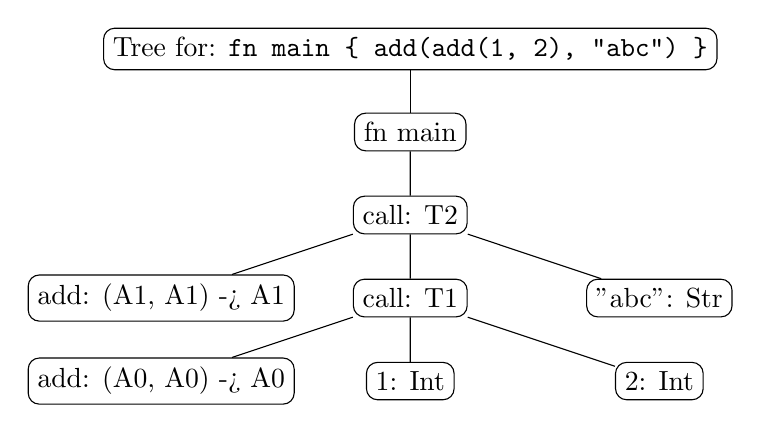
\begin{tikzpicture}[
  sibling distance=9em,
  level distance=3em,
  every node/.style = {shape=rectangle, rounded corners, draw, align=center}
]
  \node {Tree for: \verb|fn main { add(add(1, 2), "abc") }|}
          child {node {fn main}
              child {node {call: T2}
                    child {node {add: (A1, A1) -> A1}}
                    child {node {call: T1}
                        child {node {add: (A0, A0) -> A0}}
                        child {node {1: Int}}
                        child {node {2: Int}}
                    }
                    child {node {"abc": Str}}
              }
          };
\end{tikzpicture}
\end{frame}
  
\begin{frame}[containsverbatim]
\frametitle{How Does Spade Typecheck?}
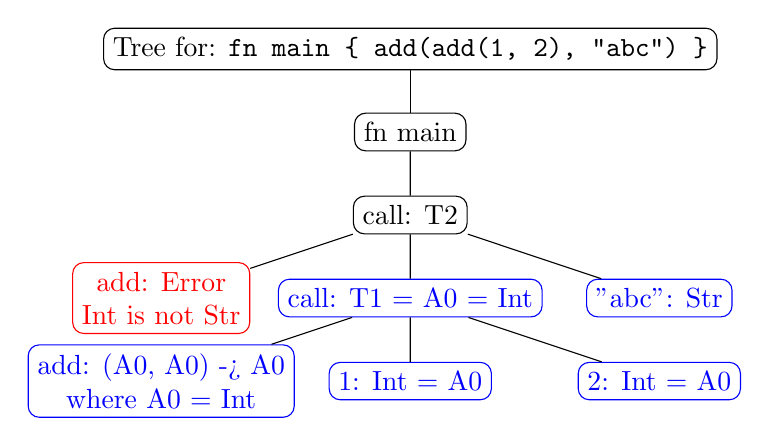
\begin{tikzpicture}[
  sibling distance=9em,
  level distance=3em,
  every node/.style = {shape=rectangle, rounded corners, draw, align=center}
]
  \node {Tree for: \verb|fn main { add(add(1, 2), "abc") }|}
          child {node {fn main}
              child {node {call: T2}
                    child {node[color=red] {add: Error\\Int is not Str}}
                    child {node[color=blue] {call: T1 = A0 = Int}
                        child {node[color=blue] {add: (A0, A0) -> A0\\where A0 = Int}}
                        child {node[color=blue] {1: Int = A0}}
                        child {node[color=blue] {2: Int = A0}}
                    }
                    child {node[color=blue] {"abc": Str}}
              }
          };
\end{tikzpicture}
\end{frame}

\begin{frame}
\frametitle{A Bit of a Breather}
\centering
The typechecker is blind to context -- it reasons locally -- all we give it is wordlength. \\[2em]
\pause
Questions about compilers or anything else?
\end{frame}

\begin{frame}[containsverbatim]
\begin{block}{Wordlength}
The number of bits a number takes in computer memory.
\centering
\begin{verbatim}
trunc<4, 3>(sb1010) =   sb010 = 2
 sext<4, 5>(sb1010) = sb11010 = -6
 zext<4, 5>(sb1010) = sb01010 = 10
\end{verbatim}
\end{block}
\end{frame}

\subsection{Self Validating Numerical Methods}

\begin{frame}
\frametitle{IA -- Interval Arithmetic}

\begin{block}{Idea}
Keep track of lowest and highest point
\end{block}

\begin{enumerate}
  \item $n \times [a, b] = [n \times a, n \times b]$
  \item $[a, b] - [c, d] = [a - d, b - c])$
  \item $[a, b] + [c, d] = [a + c, b + d]$
\end{enumerate}
\end{frame}

\begin{frame}
\frametitle{IA -- Interval Arithmetic, Example}

Given $x = [0, 1], z = [1, 3]$
\begin{align*}
  2x + z - z \\
  =^{\text{expansion}} \quad & 2 \times [0, 1] + [1, 3] - [1, 3] \\
  =^{1}                \quad & [2 \times 0, 2 \times 1] + [1, 3] - [1, 3] \\
  =^{2}                \quad & [0, 2] + [1 - 3, 3 - 1] \\
  =^{\text{simplify}}  \quad & [0, 2] + [-2, 2] \\
  =^{3}                \quad & [0 + -2, 2 + 4] \\
  =^{\text{simplify}}  \quad & [2, 4]
\end{align*}
\end{frame}

\begin{frame}
\frametitle{IA -- Interval Arithmetic, Notes}

\begin{itemize}
  \item A rigorous framework for overestimation
  \item Has no memory and struggles with $a - a$
  \item Very simple
  \item Handles 0s with care
  \item Not a field
\end{itemize}
\end{frame}

\begin{frame}
\frametitle{AA -- Affine Arithmetic}

\begin{block}{Idea}
Track some concept of variables
\end{block}

\begin{enumerate}
  \item $[a, b] \Rightarrow x_0 = (a + b) / 2, x_n = (a - b) / 2$ where $n$ is unique, this maps a range to its affine form $\hat{x}$
  \item $n \times \hat{x} = \hat{z}$ where $z_n = n \times x_n$
  \item $-\hat{x} = \hat{z}$ where $z_n = -x_n$
  \item $\hat{x} + \hat{y} = \hat{z}$ where $z_n = x_n + y_n$
  \item $\hat{x} \Rightarrow [a, b]$ where $a = x_0 + \sum_{1\dots{}n}{x_ie_i}: e_n = -1$ and $b = x_0 + \sum_{1\dots{}n}{x_ie_i}: e_n = 1$
\end{enumerate}
\end{frame}

\begin{frame}
\frametitle{AA -- Affine Arithmetic, Example}

Given $x = [0, 1], z = [1, 3]$
\begin{align*}
    2x + z - z \\
    =^{\text{expansion}} \quad & 2 \times (0.5 + 0.5e_x) + (2 + e_z) - (2 + e_z) \\
    =^{2} \quad & (1 + e_x) + (2 + e_z) - (2 + e_z) \\
    =^{3} \quad & (1 + e_x) + (2 + e_z) + (-2 + -e_z) \\
    =^{4} \quad & (3 + e_x + e_z) + (-2 + -e_z) \\
    =^{4} \quad & (1 + e_x + 0e_z) \\
    \Rightarrow^{5} \quad & [1 - 1 - 0, 1 + 1 + 0] = [0, 2]\\
\end{align*}
\end{frame}

\begin{frame}
\frametitle{AA -- Affine Arithmetic, Notes}

\begin{itemize}
  \item A rigorous framework for overestimation
  \item Has some memory
  \item Multiplication adds noise ($\hat{a}\times\hat{b} - \hat{a}\times\hat{b} \not{=} 0$)
  \item More complex
  \item Careless about 0s due to noise
  \item Not a field
\end{itemize}
\end{frame}

\subsection{FPGAs}
\begin{frame}
\frametitle{What You Need To Know About FPGAs}

\begin{itemize}
  \item \say{Programmable hardware}
  \item Builds circuits so it makes sense to have a 5 bit integer
  \item Has to be layouted on a chip
  \item Syntehsis and place-and-route is nondeterministic
  \item Uses lookup-tables (LUTs) for boolean functions
  \item Used in cars and weapons 
\end{itemize}
\end{frame}


%%%%%%%%%%%%%%%%%%%%%%%%%%%%%%

\section{The Solution(s)}

\begin{frame}
\frametitle{The Solutions Tried In This Thesis}

\centering
\begin{tabular}{l c}
 \multicolumn{2}{c}{Inside Typechecker} \\
 \hline
 1, 2 & Modifying Constraints \\
 3 & Adding New Constraints \\
 4 & Adding Missing Information \\
 5, 6 & Verifying Hypothisis \\[2em]

 \multicolumn{2}{c}{Seperate Module} \\
 \hline
 7 & A Simple Prototype \\
 7+ & Extending Into Syntax \\
\end{tabular}
\end{frame}

\subsection{7th Attempt}

\begin{frame}[containsverbatim]
\frametitle{High Level Details of 7th Attempt}
\begin{enumerate}
  \item Disable the old wordlength inference
  \item Construct equations from all integer expressions
  \item Run a SAT-solver on the equations 
  \item Inject the equations into the typesystem
\end{enumerate}
\end{frame}

\begin{frame}[containsverbatim]
\frametitle{Construct Equations and SAT-solve Example}
\begin{center}
\begin{minted}[]{rust}
fn f(a: int<4>) -> int<_> {
  let b = a + 4;
  a + b
}
\end{minted}
\begin{tabular}{l c l c l}
 Definitions & & Equations & & IA Solved \\
 $a : \textrm{int<}4\textrm{>}$ & & $r(a) = -8..8$ & & $r(a) = -8..8$ \\
 $b = a + 4$ & $\Rightarrow$ & $r(b) = r(a) + 4..4$ & $\Rightarrow$ & $r(b) = -4..12$\\
 $c = a + b$ & & $r(c) = r(a) + r(b)$ & & $r(c) = -12..20$ \\
\end{tabular}
\end{center}
\end{frame}

\begin{frame}[containsverbatim]
\footnotesize
\frametitle{This Works and We Can Now Type-check This Code}
\begin{minted}[]{rust}
// Old Spade wordlength inference
fn add_and_subtract(x: int<5>) -> int<8> {
  (x - x) + (x - x) + sext(x - x)
}

// New Spade wordlength inference using AA
fn add_and_subtract(x: int<5>) -> int<0> {
  (x - x) + (x - x) + (x - x)
}
\end{minted}
\end{frame}

\begin{frame}[containsverbatim]
\footnotesize
\frametitle{The Number of LUTs}
\begin{table}[h!]
\begin{center}
\begin{tabular}{l | c c c}
  & OLD (Old version) & IA & AA \\
\hline
Average number of LUTs&179.6&176.9 & 177.1 \\
Variance for number of LUTs &13.2&6.0&8.2 \\
Largest number or LUTs&186.0&181.0&183.0 \\
Smallest number of LUTs&171.0&171.0&167.0 \\
\end{tabular}\\[2em]
Synteshsis and PNR for the \verb`spade-memory-display` with different versions of wordlength inference.
\end{center}
\end{table}
\end{frame}

\begin{frame}[containsverbatim]
\footnotesize
\frametitle{The Number of LUTs}
\begin{table}[h!]
\begin{center}
\begin{tabular}{l | c c c}
  & OLD (Old version) & IA & AA \\
\hline
Variance for number of LUTs &13.2&6.0&8.2 \\
\end{tabular}\\[2em]
\end{center}
\end{table}
\end{frame}

\begin{frame}
\begin{center}
\LARGE But why stop here?
\end{center}
\end{frame}

\subsection{7+}

\begin{frame}
\frametitle{The 7+}

\begin{itemize}
  \item Proposed syntax change
  \item Combine AA and IA to get something better
  \item MORE DATA
\end{itemize}
\end{frame}

\begin{frame}[containsverbatim]
\frametitle{Proposed Syntax Change - Ranges In Types}

\small
\begin{minted}[]{rust}
fn twice<#A, #B, #M, #N>(x: int<A..B>) -> int<M..N> {
  2 * x
}

fn add_one<#A, #B, #M, #N>(x: int<A..B>) -> int<M..N> {
  x + 1
}

entity main(clk: clock, rst: bool) -> int<14..14> {
  let a: int<6..6> = twice(3);
  let b: int<7..7> = add_one(a);
  let c: int<14..14> = twice(b);
  c
}
\end{minted}
\end{frame}

\begin{frame}[containsverbatim]
\frametitle{Combine AA and IA (AAIA)}
\begin{itemize}
  \item AA is good at addition
  \item IA respects 0
  \item Combination is strictly better
\end{itemize}
\end{frame}

\begin{frame}[containsverbatim]
\begin{center}

\includegraphics[height=0.9\paperheight]{figures/meme.jpg}
\end{center}
\end{frame}

\begin{frame}[containsverbatim]
\frametitle{IA, AA and AAIA comparison table (OF DOOM)}
\footnotesize
\begin{tabular}{l | c c c}
                                  & IA     & AA     & AAIA    \\
                                  & \multicolumn{3}{c}{Input Wordlength $= 5$} \\
  \hline
  $a - a + a - a + a - a$   & $-93..93$ & $0..0$          & $0..0$       \\
  $(a - b) \cdot (b - a)$\footnote[2]{This row is wrong, $(a - b) \cdot (b - a) = -a^2 -b^2 \not{=} 0$} & $-961..961$ & $0..0$           & $0..0$       \\
  $a \cdot a \cdot b \cdot b \cdot c \cdot c$\footnote[1]{Results in this row are rounded to fit in the slide} & $-1.5E7..1.6E7$      & $-1.6E7..1.6E7$      & $-1.5E7..1.6E7$ \\[0.7em]
                                  & \multicolumn{3}{c}{Input Range $= 0..100$} \\
  \hline
  $a - a + a - a + a - a$   & $-300..300$ & $0..0$          & $0..0$       \\
  $(a - b) \cdot (b - a)$\footnote[4]{Also wrong}             & $-10000..10000$ & $0..0$           & $0..0$       \\
  $a \cdot a \cdot b \cdot b \cdot c \cdot c$         & $0..10^{12}$      & $-9.6875^{12}..10^{12}$      & $0..10^{12}$
\end{tabular}
\end{frame}

\begin{frame}[containsverbatim]
\frametitle{MORE DATA with the FIR filter}
\begin{itemize}
  \item IA: \verb+int<0..400000>+
  \item AA: \verb+int<-200000..400000>+
  \item AAIA: \verb+int<0..400000>+
\end{itemize}
The return types for a simple FIR-filter test program where the wordlength inference method was varied.
\end{frame}

\section{Conclusions}

\begin{frame}[containsverbatim]
\frametitle{Conclusions}
\begin{itemize}
  \item This is possible
  \item FPGA  optimizations also help
  \item Messing with codegen might make a big difference
  \item The code has atleast 1 bug
  \item Pave the way for more language features in Spade
\end{itemize}
\end{frame}

\section{Questions}

\begin{frame}[containsverbatim]
\begin{center}
\Large

\includegraphics[height=3em]{figures/spadefish.png}\\[2em]

\includegraphics[width=\textwidth]{figures/wordart.png}\\[2em]
\reflectbox{
\includegraphics[height=3em]{figures/spadefish.png}}
\end{center}
\end{frame}

\begin{frame}[containsverbatim]
\frametitle{Multiplication for IA}
\footnotesize
\begin{minted}{python}
def Addition(A..B, P..Q):
  (A + P)..(B + Q)

def Multiplication(A..B, P..Q):
  Min(A * Q, A * P, B * Q, B * P)..Max(A * Q, A * P, B * Q, B * P)

def Negation(A..B):
  -B..-A
\end{minted}
\end{frame}

\begin{frame}[containsverbatim]
\frametitle{Multiplication for AA}
\footnotesize
\begin{minted}{python}
def Rad(A):
  Sum(A[/0])

def Addition(A, B):
  [I: (A[I] or 0) + (B[I] or 0) for I in (Indices(A) U Indices(B))]

def Multiplication(X, Y):
  P = RangeToAAF(Range::Multiplication(X[0]..X[0], Y[0]..Y[0]))
  Affine(X, Y, Y[0], X[0], -P[0], (Rad(X) * Rad(Y)) + Rad(P))

def Affine(X, Y, Alpha, Beta, Gamma, Delta)
  Z = [I:   Alpha * (X[I] or 0)
          + Beta  * (Y[I] or 0)
          + (Gamma if I == 0 else 0)
        for I in Union(Indices(X), Indices(Y))]
  Z[NewUniqueIndex()] = Delta
  Z
\end{minted}
\end{frame}

\begin{frame}[containsverbatim]
\footnotesize
\frametitle{The Broad Strokes of the Seperate Module}
\begin{minted}[]{python}
(Variables, Equations) = VisitAllIntegerExpressions(AST, TypeChecker)
# We ask the typesystem for its sizes where we have known types
Known = ExtractKnownWordlengths(Variables, AST)

for _ in Equations:
  KnownAtStart = Clone(Known)
  for (Var, Body) in Equations:
    OptionRange = match InferMethod:
                  IA -> EvaluateUsingIa(Known, Body)
                  AA -> EvaluateUsingAa(Known, Body)
    match OptionRange:
      Some(Range) -> InjectAndCheckForContradictions(Range, Known)
      None -> pass
  # If we did not progress we abort
  if KnownAtStart == Known:
    break
\end{minted}
\end{frame}


\end{document}

